% !TeX program = pdfLaTeX
\documentclass[smallextended]{svjour3}       % onecolumn (second format)
%\documentclass[twocolumn]{svjour3}          % twocolumn
%
\smartqed  % flush right qed marks, e.g. at end of proof
%
\usepackage{amsmath}
\usepackage{graphicx}
\usepackage[utf8]{inputenc}

\usepackage[hyphens]{url} % not crucial - just used below for the URL
\usepackage{hyperref}
\providecommand{\tightlist}{%
  \setlength{\itemsep}{0pt}\setlength{\parskip}{0pt}}

%
% \usepackage{mathptmx}      % use Times fonts if available on your TeX system
%
% insert here the call for the packages your document requires
%\usepackage{latexsym}
% etc.
%
% please place your own definitions here and don't use \def but
% \newcommand{}{}
%
% Insert the name of "your journal" with
% \journalname{myjournal}
%

%% load any required packages here



\usepackage{booktabs}
\usepackage{longtable}
\usepackage{array}
\usepackage{multirow}
\usepackage{wrapfig}
\usepackage{float}
\usepackage{colortbl}
\usepackage{pdflscape}
\usepackage{tabu}
\usepackage{threeparttable}
\usepackage{threeparttablex}
\usepackage[normalem]{ulem}
\usepackage{makecell}
\usepackage{xcolor}

\begin{document}

\title{Accuracy and precision of zero-heat-flux temperature monitoring: a
systematic review and meta- analysis \thanks{Grants or other notes about the article that should go on the front page
should be placed here. General acknowledgments should be placed at the
end of the article.} }


    \titlerunning{Accuracy of zero-heat-flux temperature monitoring}

\author{  Aaron Conway \and  Navpreet Kamboj \and  }

    \authorrunning{ Conway }

\institute{
        Aaron Conway \at
     Peter Munk Cardiac Centre, UHN \& Lawrence S. Bloomberg Faculty of
 Nursing, University of Toronto \\
     \email{\href{mailto:aaron.conway@utoronto.ca}{\nolinkurl{aaron.conway@utoronto.ca}}}  %  \\
%             \emph{Present address:} of F. Author  %  if needed
    \and
        Navpreet Kamboj \at
     Lawrence S. Bloomberg Faculty of Nursing, University of Toronto \\
     \email{\href{mailto:navpreet.kamboj@mail.utoronto.ca}{\nolinkurl{navpreet.kamboj@mail.utoronto.ca}}}  %  \\
%             \emph{Present address:} of F. Author  %  if needed
    \and
    }

\date{Received: date / Accepted: date}
% The correct dates will be entered by the editor


\maketitle

\begin{abstract}
The text of your abstract. 150 -- 250 words.
\\
\keywords{
        key \and
        dictionary \and
        word \and
    }


\end{abstract}


\def\spacingset#1{\renewcommand{\baselinestretch}%
{#1}\small\normalsize} \spacingset{1}


\hypertarget{introduction}{%
\section{Introduction}\label{introduction}}

Core temperature monitoring is an important intervention within
perioperative and intensive care settings. Thermoregulatory dysfunction
is commonly associated with the induction of anesthesia and can lead to
adverse outcomes including cardiac dysrhythmias, altered hemostasis and
increased risk of surgical site infection (Frank et al. 1997; Kurz,
Sessler, and Lenhardt 1996; Michelson et al. 1994; Rohrer and Natale
1992). The pulmonary artery catheter is the reference standard for
continuous core temperature monitoring, however, the invasive nature of
this method renders an increased risk of bloodstream infections and
damage to surrounding tissue(Hadian and Pinsky 2006). Although
clinically accurate relative to pulmonary artery temperature
measurements, surrogate measures of core temperature at esophageal,
rectal, and bladder locations remain mildly invasive interventions.

Zero-heat-flux thermometry is an alternative non-invasive method that
allows for continuous monitoring of core temperature. Originally
developed in the 1970s, zero-heat-flux technology was recently
implemented in the 3M SpotOn temperature monitoring system (3M, St Paul,
MN), as a single-use, disposable sensor. In practice, the zero-heat-flux
sensor, such as the 3M SpotOn, is placed on the lateral surface of the
forehead and isinitially warmed to equilibrate the temperature of the
skin surface to the underlaying core tissues. Equipped with a thermal
insulator, the zero-heat-flux sensor eliminates heat loss to the
environment to allow for changes in core temperature to be directly
reflected by a change in skin surface temperature (Eshraghi et al.
2014).

The agreement between zero-heat-flux thermometers and core as well as
other peripheral thermometers has been investigated in multiple studies
over the last five years. Appraisal of these studies and synthesis of
the results would aid clinicians in deciding the appropriate
circumstances in which zero-heat-flux thermometers may be used. We aimed
to determine if zero-heat-flux thermometers have clinically acceptable
accuracy and precision relative to established core and peripheral
temperature measurement devices. Accuracy is defined as the average
difference between temperature measurements from the zero-heat-flux and
comparator device and precision as the variance (standard deviation) in
the differences.

\hypertarget{methods}{%
\section{Methods}\label{methods}}

A systematic review was conducted in accordance with a predetermined
protocol. The protocol was submitted to PROSPERO for registration but
due to delays in processing we had started data extraction by the time
it was reviewed. Therefore, the protocol did not meet the requirements
for registration. A copy of the submitted protocol can be accessed
\href{https://github.com/awconway/zhf-review}{here}. The primary
comparison for this review was temperature measured from a
zero-heat-flux thermometer versus temperature measured from a core site,
which we defined as temperature measured at either an arterial,
esophaeal, bladder or rectal site. Secondary comparisons were made
between zero-heat-flux thermometers and temperatures taken at peripheral
sites.

\hypertarget{inclusion-criteria}{%
\subsection{Inclusion criteria}\label{inclusion-criteria}}

Observational studies that reported temperature measurements from a
zero-heat-flux thermometer and comparator thermometer were included.
Studies involving a case control design were excluded due to potential
for overestimation of the intervention performance. Studies were
excluded if conducted on non-human subjects or outside of a clinical
healthcare setting. No publication date restrictions were
applied.Published conference abstracts were included if there was enough
information reported to appraise the quality of the study. There were no
language restrictions applied during the search.

\hypertarget{data-sources-and-searches}{%
\subsection{Data sources and searches}\label{data-sources-and-searches}}

Published studies were found by searching Medline and EMBASE from
January 2000 to July 2019. The Cochrane-recommended search strategy
combining terms for the `target condition' and `index test' was used
(Mann and Gilbody 2012). This search strategy is an efficient approach
for systematic reviews of diagnostic test accuracy studies.(Preston et
al. 2015) We also conducted forward citation searching, by using Google
Scholar to search the citations of the first article published on the
accuracy of zero-heat-flux thermometers. The search strategies used for
each data base can be located \href{shiny\%20app}{here}. Selection of
studies was undertaken independently by two reviewers using
\href{https://www.covidence.org}{Covidence}.

\hypertarget{data-extraction-and-quality-assessment}{%
\subsection{Data extraction and quality
assessment}\label{data-extraction-and-quality-assessment}}

Information was extracted regarding study characteristics (author, year
of publication, country, design, sample size, clinical setting, numbers
studied and analyses for each outcome), population characteristics
(inclusion and exclusion criteria) and temperature measurement
characteristics (placement of sensor, timing and methods of
measurements). The outcomes that were extracted included the mean bias
(eg, accuracy) and variance (eg, SD, precision) in temperature
measurement between the zero-heat-flux and comparator thermometers. We
also extracted information about how repeated measurements were handled.
In particular we assessed whether studies: (1) analysed each pair of
data separately; (2) treated each pair of data as independent; or (3)
used either analysis of variance or a random effects model as a way to
control for the dependent nature of the repeated measures data (Myles
and Cui 2007).

Two reviewers independently assessed the risk of bias for the included
studies using the revised Quality Assessment of Diagnostic Accuracy
Studies (QUADAS-2) (Whiting et al. 2011). Reviewers rated the risk of
bias for patient selection, conduct of the zero-heat-flux measurements,
conduct of the comparator thermometer measurements, and timing and flow
(eg, timing of ZHF and established core temperature measurements,
dropouts) as ``high'', ``low'' or ``unclear'' risk of bias. We worked to
minimize the risk of publication bias by conducting a comprehensive
search of multiple databases as well as an international clinical trial
registry (Glasziou et al. 2001). Statistical approaches for detection of
reporting bias were not conducted due to lack of validated methods (Begg
2005). ASimulations have revealed that tests for detecting funnel plot
asymmetry will result in publication bias being incorrectly identified
too often (Deeks, Macaskill, and Irwig 2005).

In order to rate the quality of evidence, we applied the Grading Quality
of Evidence and Strength of Recommendation methodology (Schünemann et
al. 2008). Evidence was downgraded in accordance with study limitations,
inconsistency and imprecision. There were no circumstances in which
evidence was downgraded for indirectness as this systematic review only
included relevant studies. Although the possibility of publication bias
was not excluded, this bias was not formally assessed as it was not
considered sufficient enough to reason downgrading the quality of
evidence.

\hypertarget{data-synthesis-and-analysis}{%
\subsection{Data synthesis and
analysis}\label{data-synthesis-and-analysis}}

The objective for the meta-analysis was to estimate the population
limits of agreement between temperature measurements from the ZHF and
established comparator thermometers. A framework for meta-analysis of
Bland-Altman method comparison studies developed by Tipton and Shuster
(2017) based on limits of agreement approach was used. This method was
selected because it parallels the approach used in primary Bland-Altman
studies, whereby an estimate is generated for the pooled LoAs in the
population (not just in the samples studied). The `population LoA' is
more broad than the LoA commonly reported in the meta-analyses of
Bland-Altman studies (Tipton and Shuster 2017). Pooled limits of
agreement were calculated using \(\delta\pm2\sqrt{\sigma2+\tau2}\),
where \(\delta\) is the average bias across studies, \(\sigma2\) is the
average within-study variation in differences and \(\tau2\) is the
variation in bias across studies.

Estimations of \(\delta\) and \(\sigma2\) were made using a weighted
least-squares model (similar to a random-effects approach), with the
associated standard errors estimated using robust variance estimation.
Robust variance estimation was used alternatively to model-based
standard errors as some studies included in the systematic review used
repeated-measures designs without accommodating for the correlation
between measurements (Hedges, Tipton, and Johnson 2010; Tanner-Smith,
Tipton, and Polanin 2016; Tipton 2015). We used the method-of-moments
estimator from DerSimonian and Laird (1986) for the \(\tau2\) parameter.

Measures of uncertainty were included in our meta-analyses by
calculating the outer \(95\%\) confidence intervals for pooled limits of
agreement. We also accounted for repeated measurements if they were not
properly adjusted for in individual studies. This was achieved by using
weights proportional to the number of participants, not the total number
of measurements. The R statistical program was used to conduct all
analyses (Team 2017). All data and R code used in the meta-analyses can
be located \href{}{here}.

Prior to conducting the meta-analyses, the results from each study were
converted into a standard format, with bias meaning
\(comparator thermometer-ZHF thermometer\) measured in \(^\circ C\). In
several studies, results were reported for multiple groups of
participants, therefore in the meta-analysis each of these groups was
treated as a separate `comparison'. Other studies reported multiple sets
of results, whereby analyses were conducted between ZHF and various
comparator devices used on the same participant. These instances were
also treated as a separate `comparison' if the comparator devices were
apart of separate meta-analyses groups. One study reported
intraoperative, postoperative and overall results for the same
participants. Only the paired measurements from the overall results were
included in the main and low risk bias analyses, leaving paired
measurements exclusively from the intraoperative and postoperative
timepoints to be included in respective meta-analyses subgroups.

The conventionally cited clinically acceptable agreement between ZHF and
comparator devices is 0.5 \(^\circ C\)
\((ref - most of the studies site this range from Eshragi...)\). It was
deemed that outer confidence bounds for 95\% LoA between zero-heat-flux
and core temperature measurements (termed as `population limits of
agreement') outside of these bounds wouldbe clinically unacceptable.

A sensitivity analysis for the primary comparison (ZHF versus
temperature measurement at core site) was performed based on risk of
bias, whereby `unclear risk of bias' was treated as `high risk' and
`high risk of bias' studies were excluded from analyses. As clinicians
would be interested in the accuracy of ZHF relative to the thermometer
devices they use, and within the clinical setting in which they use it,
we conducted subgroup analyses according to the comparator device used
(either core, sublingual or nasopharangeal) and clinical setting (either
intraoperative or intensive care unit).

\hypertarget{results}{%
\section{Results}\label{results}}

\hypertarget{study-selection-and-description}{%
\subsection{Study selection and
description}\label{study-selection-and-description}}

Fifteen studies were included (Figure 1). Two studies reported only in
abstract form were not included and assigned as `studies awaiting
classification' because there was insufficient information provided.

\begin{figure}

{\centering 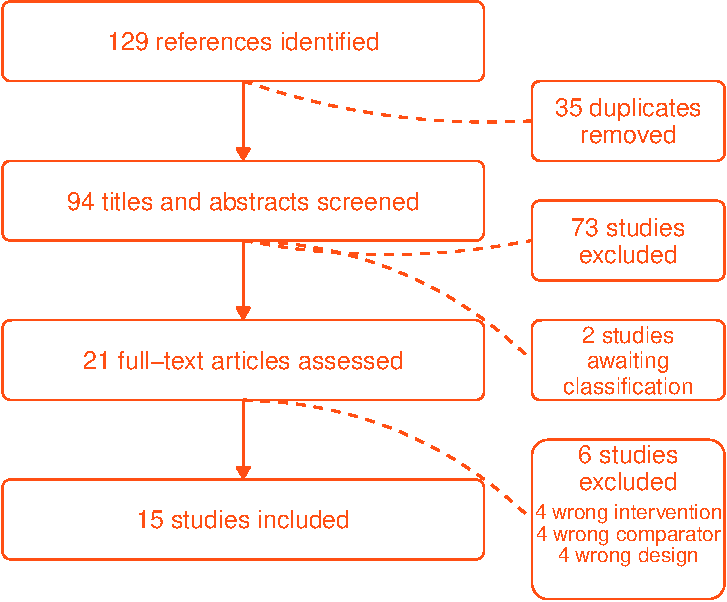
\includegraphics{fig-1-1} 

}

\caption{PRISMA Flow Diagram}\label{fig:fig-1}
\end{figure}

The characteristics of included studies can be viewed
\href{link\%20to\%20shiny\%20app}{here}. The primary comparison of
zero-heat-flux versus core temperature measurements (eg, arterial,
bladder, esophageal or rectal) consisted of 19 comparisons from 13
individual studies. In total, data from 576 participants with 179,821
paired measurements were included in this comparison (two studies did
not report the total number of measurements included in their analysis).
The sensitivity analysis for the primary comparison with only studies
that were judged as low risk of bias across all domains included 10
comparisons from 5 studies that enrolled 273 participants with 104,294
paired measurements (two studies did not report the total number of
measurements included in their analysis). There were 5 studies that
compared zero-heat-flux to core temperature measurements in ICU
patients, comprising 7 comparisons with 155,598 measurements from 246
participants. Another 9 studies were included that compared
zero-heat-flux to core temperature measurements in patients undergoing
surgery, comprising 13 comparisons with 24,223 measurements from 433
participants. Nasopharyngeal thermometers were used as the comparator
devices in 4 studies, with 109,819 paired measurements from 109,819
participants. Sublingual thermometers were used as the comparator
devices in 2 studies that reported 22,731 paired measurements from 107
participants.

All studies included in this systematic review evaluated the
zero-heat-flux temperature monitoring system manufactured by 3M.
Previously known as the SpotOn Temperature Monitoring System, the 3M ZHF
device is now referred to commercially as the Bair Hugger Temperature
Monitoring System. All comparisons reported adherence to the
zero-heat-flux device manufacturer instructions and placed the sensor on
the forehead of the participants. One included study also reported
results for a comparison where the zero-heat-flux thermometer was placed
on the forehead. We did not included this comparison in our
meta-analysis.

High risk of bias was associated with patient selection for 13 (43\%)
comparisons from 9 (56\%) studies, conduct of ZHF and comparator
measurements in 10(33\%) comparisons from 8 (50\%) studies and 12 (40\%)
comparisons 9 (30\%) studies, respectively (mostly due to ZHF
measurements being taken with knowledge of the comparator measurements
and vice versa) and participant flow for 13 (43\%) studies. In 19 (50\%)
comparisons from 8 (50\%) studies, the authors had declared a conflict
of interest or receipt of funding or equipment from the manufacturer of
the ZHF device under evaluation.

\hypertarget{primary-comparison-zero-heat-flux-thermometer-versus-core-thermometers}{%
\subsection{Primary comparison: zero-heat-flux thermometer versus core
thermometers}\label{primary-comparison-zero-heat-flux-thermometer-versus-core-thermometers}}

The pooled estimate for the mean bias between zero-heat-flux and core
temperature measurements was 0\(^\circ C\). However, the variation in
differences between studies was large, as displayed by the density plot
in Figure 2. Consequently, the population limits of agreement, which
take into consideration the between-study heterogeneity and sampling
error, were wide, spanning from -1\(^\circ C\) to 1.1\(^\circ C\)
(179,821 measurements; 576 participants; 13 studies). The quality of
evidence for the primary comparison was downgraded to low quality due to
concerns about study limitations and inconsistency. Population limits of
agreement for the sensitivity analysis restricted to studies rated as
having low risk of bias across all the domains of the QADAS-2 were
similar to the primary analysis (104,294 measurements; 273 participants;
5 stsudies). The mean bias was again 0\(^\circ C\) with population
agreements spanning from -1\(^\circ C\) to 1.1\(^\circ C\).

\begin{figure}

{\centering 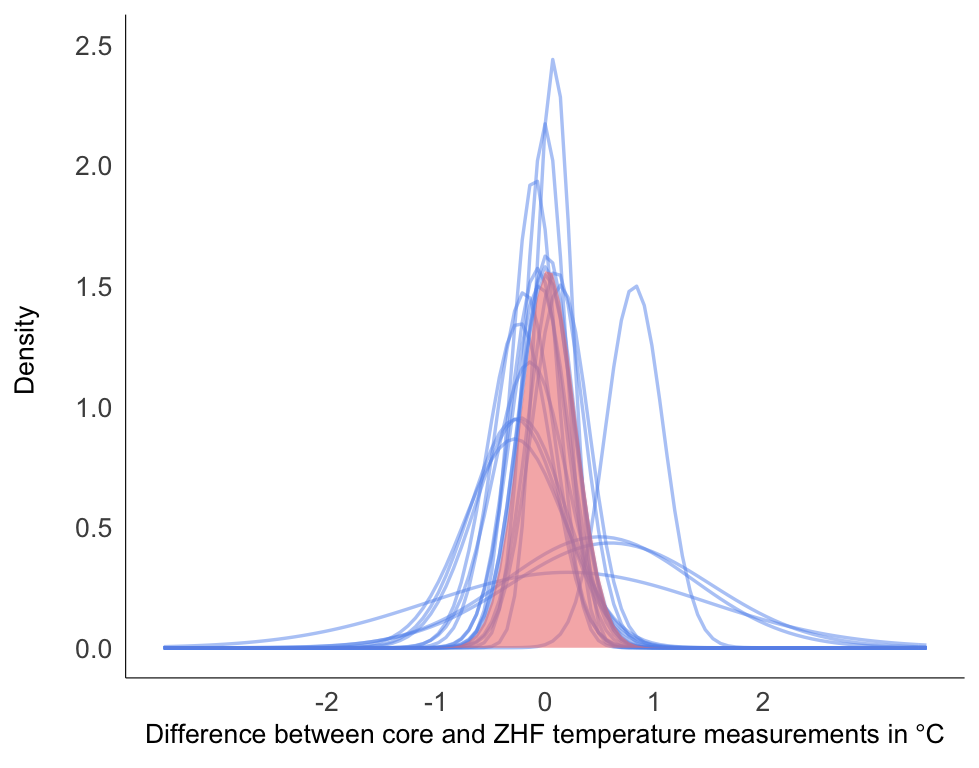
\includegraphics{fig-2-1} 

}

\caption{Comparisons between core and zero-heat-flux thermometers within and across studies. Blue curves are distributions of the differences between measurements from zero-heat-flux (ZHF) sensors and core temperature measurements in individual studies. The red curve is the distribution of the pooled estimate.}\label{fig:fig-2}
\end{figure}

We conducted two subgroup analyses for the primary comparison according
to the clinical setting in which the study was conducted. In the subset
of studies conducted in the ICU, the mean bias was 0 \(^\circ C\) with
population limits of agreement between -1.5 \(^\circ C\) and 1.4
\(^\circ C\). Whereas in the subset of studies that evaluated the use of
zero-heat-flux thermometers during surgery found a mean bias of 0
\(^\circ C\) with population limits of agreement from -1.1 \(^\circ C\)
to 1.1 \(^\circ C\). The quality of evidence for these subgroup analyses
was similarly rated as low quality due to concerns about study
limitations and inconsistency.

\hypertarget{secondary-comparisons-zero-heat-flux-thermometer-versus-peripheral-thermometers}{%
\subsection{Secondary comparisons: zero-heat-flux thermometer versus
peripheral
thermometers}\label{secondary-comparisons-zero-heat-flux-thermometer-versus-peripheral-thermometers}}

Zero-heat-flux thermometers were compared with sublingual thermometers
and nasopharyngeal thermometers in the studies included in this review.
The mean bias between zero-heat-flux and sublingual temperature
measurements in meta-analysis of results from 2 studies was -0.2
\(^\circ C\). Due to the limited number of studies and measurements,
population limits of agreement were extremely wide, spanning from -13.3
\(^\circ C\) to 12.8 \(^\circ C\). The quality of evidence for this
comparison was rated as very low quality due to serious concerns about
imprecision.

The mean bias between zero-heat-flux and nasopharyngeal temperature
measurements in meta-analysis of results from 4 studies was 0
\(^\circ C\). Population limits of agreement were -1 \(^\circ C\) to 1
\(^\circ C\). We downgraded the quality of evidence to low, again due to
concerns about inconsistency and study limitations.

\hypertarget{discussion}{%
\section{Discussion}\label{discussion}}

Results from this systematic review have important implications for
practice. Clinicians should consider the potential that a temperature
measurement from a zero-heat-flux thermometer could be as much as one
\(^\circ C\) higher or lower than the true core temperature. This is
similar to results from previous meta-analyses that compared other
peripheral thermometers with core temperature measurements. However,
these previous meta-analyses used statistical approaches that did not
incorporate the magnitude of heteroogeneity in results between studies
or sampling error. As such, it is possible that the zero-heat-flux
thermometer is still more precise than these other peripheral
thermometers.

Whether or not teh zero-heat-flux thermometer is sufficiently accurate
to be used in place of nasopharyngeal thermometers is unclear.

\hypertarget{limitations}{%
\subsection{Limitations}\label{limitations}}

\hypertarget{conclusion}{%
\section{Conclusion}\label{conclusion}}

\hypertarget{references}{%
\section*{References}\label{references}}
\addcontentsline{toc}{section}{References}

\hypertarget{refs}{}
\leavevmode\hypertarget{ref-begg2005systematic}{}%
Begg, Colin B. 2005. ``Systematic Reviews of Diagnostic Accuracy Studies
Require Study by Study Examination: First for Heterogeneity, and Then
for Sources of Heterogeneity.'' \emph{Journal of Clinical Epidemiology}
58 (9). Elsevier Limited: 865.

\leavevmode\hypertarget{ref-deeks2005performance}{}%
Deeks, Jonathan J, Petra Macaskill, and Les Irwig. 2005. ``The
Performance of Tests of Publication Bias and Other Sample Size Effects
in Systematic Reviews of Diagnostic Test Accuracy Was Assessed.''
\emph{Journal of Clinical Epidemiology} 58 (9). Elsevier: 882--93.

\leavevmode\hypertarget{ref-dersimonian1986meta}{}%
DerSimonian, Rebecca, and Nan Laird. 1986. ``Meta-Analysis in Clinical
Trials.'' \emph{Controlled Clinical Trials} 7 (3). Elsevier: 177--88.

\leavevmode\hypertarget{ref-eshraghi2014}{}%
Eshraghi, Yashar, Vivian Nasr, Ivan Parra-Sanchez, Albert Van Duren,
Mark Botham, Thomas Santoscoy, and Daniel I Sessler. 2014. ``An
Evaluation of a Zero-Heat-Flux Cutaneous Thermometer in Cardiac Surgical
Patients.'' \emph{Anesthesia \& Analgesia} 119 (3). LWW: 543--49.

\leavevmode\hypertarget{ref-frank1997perioperative}{}%
Frank, Steven M, Lee A Fleisher, Michael J Breslow, Michael S Higgins,
Krista F Olson, Susan Kelly, and Charles Beattie. 1997. ``Perioperative
Maintenance of Normothermia Reduces the Incidence of Morbid Cardiac
Events: A Randomized Clinical Trial.'' \emph{Jama} 277 (14). American
Medical Association: 1127--34.

\leavevmode\hypertarget{ref-glasziou2001systematic}{}%
Glasziou, Paul, Les Irwig, Chris Bain, and Graham Colditz. 2001.
\emph{Systematic Reviews in Health Care: A Practical Guide}. Cambridge
University Press.

\leavevmode\hypertarget{ref-hadian2006evidence}{}%
Hadian, Mehrnaz, and Michael R Pinsky. 2006. ``Evidence-Based Review of
the Use of the Pulmonary Artery Catheter: Impact Data and
Complications.'' \emph{Critical Care} 10 (3). BioMed Central: S8.

\leavevmode\hypertarget{ref-hedges2010robust}{}%
Hedges, Larry V, Elizabeth Tipton, and Matthew C Johnson. 2010. ``Robust
Variance Estimation in Meta-Regression with Dependent Effect Size
Estimates.'' \emph{Research Synthesis Methods} 1 (1). Wiley Online
Library: 39--65.

\leavevmode\hypertarget{ref-kurz1996perioperative}{}%
Kurz, Andrea, Daniel I Sessler, and Rainer Lenhardt. 1996.
``Perioperative Normothermia to Reduce the Incidence of Surgical-Wound
Infection and Shorten Hospitalization.'' \emph{New England Journal of
Medicine} 334 (19). Mass Medical Soc: 1209--16.

\leavevmode\hypertarget{ref-mann2012should}{}%
Mann, Rachel, and Simon M Gilbody. 2012. ``Should Methodological Filters
for Diagnostic Test Accuracy Studies Be Used in Systematic Reviews of
Psychometric Instruments? A Case Study Involving Screening for Postnatal
Depression.'' \emph{Systematic Reviews} 1 (1). BioMed Central: 9.

\leavevmode\hypertarget{ref-michelson1994reversible}{}%
Michelson, Alan D, Hollace MacGregor, Marc R Barnard, Anita S Kestin,
Michael J Rohrer, and C Robert Valeri. 1994. ``Reversible Inhibition of
Human Platelet Activation by Hypothermia in Vivo and in Vitro.''
\emph{Thrombosis and Haemostasis} 72 (05). Schattauer GmbH: 633--40.

\leavevmode\hypertarget{ref-myles2007using}{}%
Myles, PS, and James Cui. 2007. ``I. Using the Bland--Altman Method to
Measure Agreement with Repeated Measures.'' Oxford University Press.

\leavevmode\hypertarget{ref-preston2015improving}{}%
Preston, Louise, Christopher Carroll, Paolo Gardois, Suzy Paisley, and
Eva Kaltenthaler. 2015. ``Improving Search Efficiency for Systematic
Reviews of Diagnostic Test Accuracy: An Exploratory Study to Assess the
Viability of Limiting to Medline, Embase and Reference Checking.''
\emph{Systematic Reviews} 4 (1). BioMed Central: 82.

\leavevmode\hypertarget{ref-rohrer1992effect}{}%
Rohrer, Michael J, and ANITA M Natale. 1992. ``Effect of Hypothermia on
the Coagulation Cascade.'' \emph{Critical Care Medicine} 20 (10):
1402--5.

\leavevmode\hypertarget{ref-schunemann2008grading}{}%
Schünemann, Holger J, Andrew D Oxman, Jan Brozek, Paul Glasziou, Roman
Jaeschke, Gunn E Vist, John W Williams, et al. 2008. ``Grading Quality
of Evidence and Strength of Recommendations for Diagnostic Tests and
Strategies.'' \emph{Bmj} 336 (7653). British Medical Journal Publishing
Group: 1106--10.

\leavevmode\hypertarget{ref-tanner2016handling}{}%
Tanner-Smith, Emily E, Elizabeth Tipton, and Joshua R Polanin. 2016.
``Handling Complex Meta-Analytic Data Structures Using Robust Variance
Estimates: A Tutorial in R.'' \emph{Journal of Developmental and
Life-Course Criminology} 2 (1). Springer: 85--112.

\leavevmode\hypertarget{ref-team2017r}{}%
Team, R Core. 2017. ``R Core Team (2017). R: A Language and Environment
for Statistical Computing.'' \emph{R Found. Stat. Comput. Vienna,
Austria. URL Http://Www. R-Project. Org/., Page R Foundation for
Statistical Computing}.

\leavevmode\hypertarget{ref-tipton2015small}{}%
Tipton, Elizabeth. 2015. ``Small Sample Adjustments for Robust Variance
Estimation with Meta-Regression.'' \emph{Psychological Methods} 20 (3).
American Psychological Association: 375.

\leavevmode\hypertarget{ref-tipton2017framework}{}%
Tipton, Elizabeth, and Jonathan Shuster. 2017. ``A Framework for the
Meta-Analysis of Bland--Altman Studies Based on a Limits of Agreement
Approach.'' \emph{Statistics in Medicine} 36 (23). Wiley Online Library:
3621--35.

\leavevmode\hypertarget{ref-whiting2011quadas}{}%
Whiting, Penny F, Anne WS Rutjes, Marie E Westwood, Susan Mallett,
Jonathan J Deeks, Johannes B Reitsma, Mariska MG Leeflang, Jonathan AC
Sterne, and Patrick MM Bossuyt. 2011. ``QUADAS-2: A Revised Tool for the
Quality Assessment of Diagnostic Accuracy Studies.'' \emph{Annals of
Internal Medicine} 155 (8). Am Coll Physicians: 529--36.

\bibliographystyle{spbasic}
\bibliography{bibliography.bib}

\end{document}
